\documentclass[tikz,border=2pt]{standalone}
\usepackage{amsmath,amssymb}
\usepackage{tikz}
\usetikzlibrary{arrows.meta,matrix}

\begin{document}
% The augmented matrix [A | b] stores the coefficients and the right-hand side of a linear
% system side by side, so row operations act on both at once.
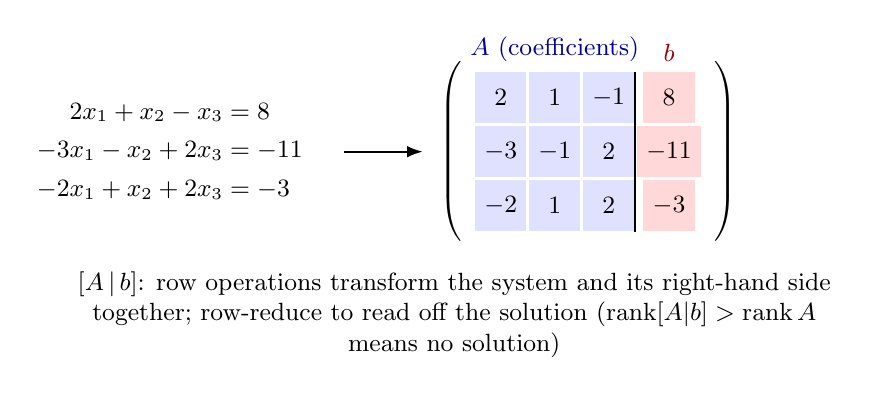
\begin{tikzpicture}[every node/.style={font=\small}, >={Latex[length=2mm]}]
	\node[anchor=east, align=left] at (-0.4,0) {$\begin{aligned}2x_1+x_2-x_3&=8\\ -3x_1-x_2+2x_3&=-11\\ -2x_1+x_2+2x_3&=-3\end{aligned}$};
	\draw[->, thick] (0,0) -- (1.0,0);
	\matrix (M) [matrix of math nodes, nodes={minimum size=6.5mm, anchor=center}, left delimiter=(, right delimiter=), column sep=1pt, row sep=1pt] at (3.1,0) {
		|[fill=blue!12]| 2 & |[fill=blue!12]| 1 & |[fill=blue!12]| -1 & |[fill=red!15]| 8 \\
		|[fill=blue!12]| -3 & |[fill=blue!12]| -1 & |[fill=blue!12]| 2 & |[fill=red!15]| -11 \\
		|[fill=blue!12]| -2 & |[fill=blue!12]| 1 & |[fill=blue!12]| 2 & |[fill=red!15]| -3 \\
	};
	\draw[thick] (M-1-3.north east) -- (M-3-3.south east);
	\node[blue!60!black, font=\small, anchor=south] at (M-1-2.north) {$A$ (coefficients)};
	\node[red!60!black, font=\small, anchor=south] at (M-1-4.north) {$b$};
	\node[anchor=north, align=flush center, text width=10cm] at (1.4,-1.4) {$[A\,|\,b]$: row operations transform the system and its right-hand side together; row-reduce to read off the solution ($\operatorname{rank}[A|b]>\operatorname{rank}A$ means no solution)};
\end{tikzpicture}
\end{document}
